%%%%%%%%%%%%%%%%%%%%%%%%%%%%%
%Since : May/13/2008
%Update: <Mar/31/2009>
%%%%%%%%%%%%%%%%%%%%%%%%%%%%%
\documentclass[12pt, a4j]{jsarticle}
\usepackage{graphicx}
\usepackage{amsmath}
\usepackage{amssymb}
\usepackage{cite}
\usepackage{listings, jlisting}
\usepackage{verbatim}
\usepackage{wrapfig}

\newcommand{\figref}[1]{図 \ref{#1}}

\title{}
\author{}
\date{}

\begin{document}

{\LARGE \bf \sf webページを作ろう}
\section{イントロ}

インターネットの普及により、大手企業だけではなく中小企業や個人も盛んにwebペー
ジを公開しています。webページは全世界に即座に情報を公開でき、しかも極めて安価
な情報媒体であるという特徴があります。非常に安価で速報性が高い媒体なので、大企業だけ
ではなく、中小企業や個人も盛んにホームページを開設し情報発信しています。

webページは初心者にも簡単に作成できます。そして、webページを作成するためには、コ
ンピュータを使う上で必要な事柄を一通り知っておく必要があります。この実験では、
webページの作成を通して、HTMLコーディング、コンピュータでのファイルの扱い方、色
の扱い方などのコンピュータを使用するための知識を総合的に学ぶことを目的とします。

\section{webページの構成}

\begin{wrapfigure}{r}{5cm}
%\begin{figure}[htbp]
\vspace{-20pt}
\begin{center}
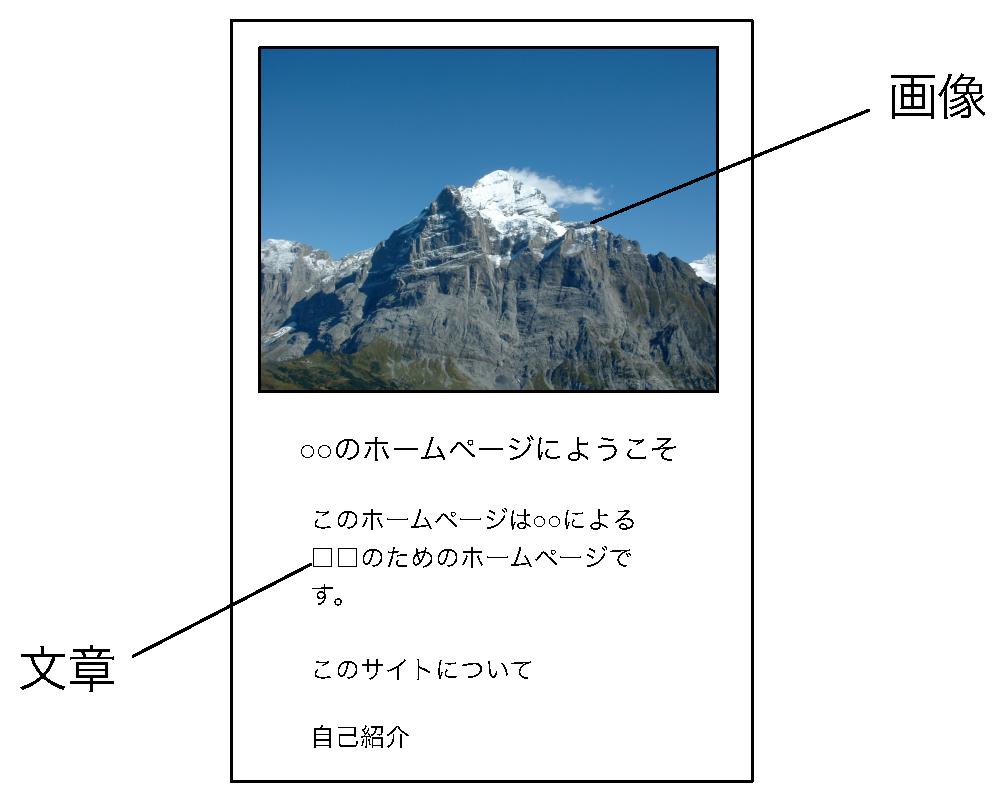
\includegraphics[width=1\linewidth]{webpage-summary.eps}
\caption{ホームページの構成}
\label{fig:summary}
\end{center}
%\end{figure}
\end{wrapfigure}
多くのホームページは、文字と画像の組み合わせでできています(\figref{fig:summary})。
さらに、動画、音楽、Flashと呼ばれるプログラムなどを組み込んだページも存在します。
ホームページを構成する文章や画像の配置などはHTML(Hyper Text Markup Language)とい
うマークアップ言語で書かれています。マークアップ言語というと専門的で難しいと
いう印象を与えるかもしれませんが、簡単なページを作るのでしたら初心者でも簡単に
できますので安心してください。


\subsection{HTML}
ホームページを作る上で基本的なファイルがHTMLファイルです。HTMLファイルはHTMLとい
うマークアップ言語で書かれています。マークアップ言語とは、どのように表示するかを
タグと呼ばれるマークを書くことにより、マークしたところをどのように表示を記述する
ための言語です。HTMLで書かれたファイルは{\bf \sf foo.html}\footnote{foo、bar、
foobar、hoge(日本限定)などは情報技術解説文やサンプルコードの中で、変数名やファイ
ル名を適当につける時に使用されるものです。IT関係の技術書やプログラムのサンプルコー
ドなどでよく見かけます。日常会話の{\bf \sf なになに}、{\bf \sf ○○}と同じ意味で
す。}もしくは{\bf \sf foo.htm}という名前で保存されています。このように、拡張子が
html, htmかどうかでそのファイルがHTMLで書かれたファイルかどうかが判断できます。

私たちが目にするホームページのすべてが(X)HTMLで書かれていますが、私たちは普
段、HTMLのコード自体を直接目にすることはないと思います。それは、HTMLファイルに書かれた
HTMLをブラウザが解釈して画面に表示してくれるからです(\figref{fig:schime})。ブラウ
ザとは、HTMLを解釈し、文字や画像を命令通り配置、装飾して画面に表示してくれるソフ
トです。ブラウザにはInternet Explore、Firefox、Operaなどがあります。

\begin{figure}[htbp]
\begin{center}
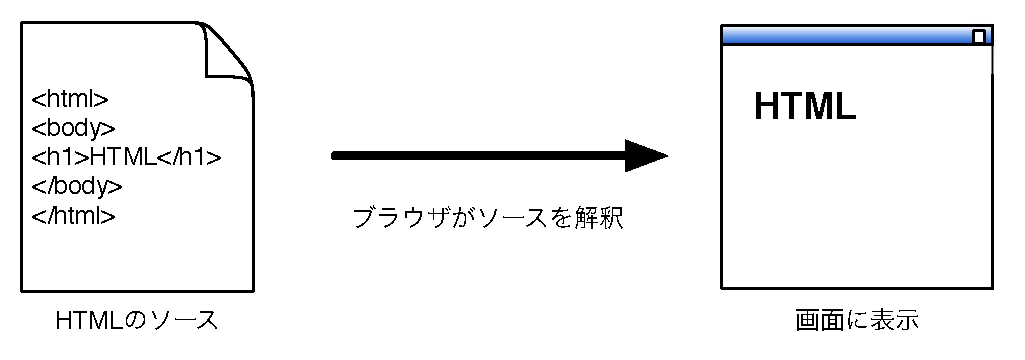
\includegraphics[width=0.8\linewidth]{img.eps}
\caption{HTMLとブラウザの関係。HTMLをブラウザが解釈して画面に表示する。}
\label{fig:schime}
\end{center}
\end{figure}


\section{webページを作る}

\subsection{HTMLファイルを扱うソフト}

HTMLファイルを扱うソフトには大きく2種類あります。ホームページを見た目のまま編集する
WYSIWYG(what you see is what you get)と呼ばれる方式のソフトと、直接
HTMLを扱うソフトがあります。WYSIWYGソフトにはホームページビルダーや
Dreamweaverなどがあります。HTMLを直接取り扱うソフトには、メモ帳、秀丸、Terapadなどのテキ
ストエディタがあります。本講座では、ホームページの構造を基礎から理解するために、HTMLを直接扱うこと
のできるメモ帳かTerapadを用います。

\subsection{本実験で使うソフト}

\begin{itemize}
    \item メモ帳かTeraPad: HTMLやプログラムソースを書くためのソフト(テキストエディタ)。
    \item InternetExplorer: ブラウザ
\end{itemize}

\subsection{手順}
ホームページの作成は下記のような手順で進めていきます。

\begin{enumerate}
\item メモ帳かTeraPad(テキストエディタ)を開く。
\item メモ帳かTeraPad(テキストエディタ)でHTMLのソースを書く。
\item 書いたソースを名前をつけて保存を選択し、保存する。
\item 保存したファイルをInternetExplorerで開き、確認する。
\item 問題があればHTMLのソースを修正し、InternetExplorerの更新ボタンを押し、確認する。
\end{enumerate}


\subsection{はじめの一歩}

では、早速ホームページを作っていきましょう。とりあえず、ソースコード1を打ち込んで
みましょう。打ち込み終わったら、保存します。保存する場合のファイル名は
``foo.html''という名前にします。fooの部分は好きな名前にしてください。保存できたら
そのファイルを開いてみましょう。開くと、動作画面のように表示されると思います。そ
こでうまく表示されない場合は打ち込みミスですので、修正し保存してブラウザの更新ボ
タンを押しましょう。

\begin{figure}[htbp]
\begin{tabular}{cc}
\begin{minipage}{0.5\hsize}
\begin{center}
\lstinputlisting[caption=サンプル]{sample.html}
\end{center}
\end{minipage}
&
\begin{minipage}{0.5\hsize}
\begin{center}
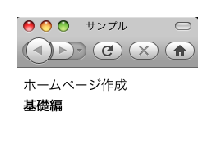
\includegraphics[width=0.8\linewidth]{sample.eps}
\caption{動作画面}
%\label{fig:1}
\end{center}
\end{minipage}
\end{tabular}
\end{figure}

\subsection{ファイル名について}

webページを作った後はそれを保存しなければなりません。
HTMLで書いたwebページのファイルは、{\bf \sf foo.html}という名前がついています。しかし、
{\bf \sf foo.html}というファイルの中には特別な役割を持ったものがあります。それは、
{\bf \sf index.html}です。ブラウザでwebページを見るときに、http://foo.bar/のようにwebペー
ジの場所(URL: Uniform Resource Locator)を指定します。URLの指定の仕方には
http://foo.bar/foobar.htmlのように直接ファイルの場所を指定するやり方とhttp://foo.bar/
のようにディレクトリの場所(Windowsでいうところのフォルダ)を指定するやり方があります。
ディレクトリの場所を指定した場合、ディレクトリの中にある{\bf \sf index.html}と名前の付
いたファイルが呼び出されます。ですので、http://foo.bar/とディレクトリを指定した
ときに開きたいページに{\bf \sf index.html}とつけるとよいでしょう。

その他に名前で注意する点があります。それはファイル名に日本語(ひらがな、カタカナ、
漢字)をつけてはいけないということです。それらの文字は、どのコンピュー
タでも解釈できるものではありません。もしそのような文字のファイル名をつけると、他の人が
webページにたどり着けなくなります。基本的にファイルの名前には半角英数文字を用い
ましょう。

\subsection{タグとは}

タグとは、テキストをどのように表示するのかを記したマークです。たとえば、{\bf \sf
$<$br$>$}というタグは改行を表します。このようにHTMLで用いられるタグは、$<$と$>$で閉じ
られています。また、{\bf \sf $<$strong$>$強調$<$/strong$>$}では、{\bf \sf
$<$strong$>$}タグで囲まれた部分が強調されます。このような、ある範囲に作用するよう
なタグは、作用させたい部分をタグで囲みます。終了を表すタグには{\bf \sf /}がつきま
す。ほかにも様々なタグが用意されています。それについては、課題1で実際にサンプルを
打ちながら学びましょう。

\subsection{HTMLのソースの構造}

\begin{wrapfigure}{r}{5cm}
%\begin{figure}[htbp]
\vspace{-35pt}
\begin{center}
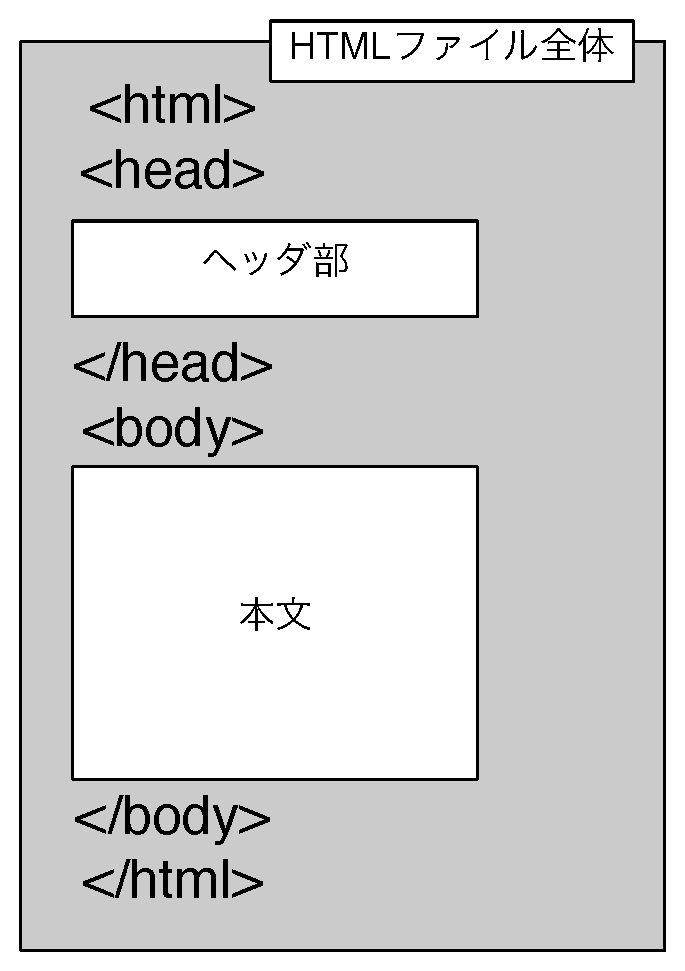
\includegraphics[width=0.6\linewidth]{structure.eps}
\caption{HTMLのソースコードの構造}
\label{fig:structure}
\end{center}
%\end{figure}
\end{wrapfigure}
HTMLのソースは\figref{fig:structure}のような構造をしています。HTMLのソースコード
は必ず{\bf \sf $<$html$>$}で囲まれます。その中に、{\bf \sf $<$head$>$}タグがあり
ます。そこには、ホームページのタイトルやJavaScriptなどを書き込みます。ホームペー
ジのタイトルは{\bf \sf $<$title$>$}タグで囲み、ウィンドウの上に表示されます。ホー
ムページの本文を書き込む場所が{\bf \sf $<$body$>$}で囲まれた部分です。基本的に、
{\bf \sf $<$body$>$}で囲まれた部分がブラウザで表示されます。


\subsection{スペースと改行}

ソースで書かれたスペースと改行は、必ずしも意図通りに表示されるとは限りません。
もし、ソースにスペースを10個書いたときいは、ブラウザで表示すると、1つしかスペー
スは表示されません。またソースに改行を10個書いたときも、スペース1つしか表示され
ません。スペースを複数表示されるには、スペースを表すタグを複数挿入しなければなり
ません。もし複数のスペースを表示したい場合は、スペースを表す{\bf \sf \&nbsp}を複数
書くことで複数のスペースを表示できます。複数の改行を表示したい場合は、前述の{\bf
\sf $<$br$>$}を複数入れると実現できます。

\subsection{色の扱い}
コンピュータでは、色をRGBで表します。RGBとは、赤(Red)、緑(Green)、青(Blue)の頭文
字をとったものです。これは、コンピュータが赤、緑、青の光の3原色で色を表しているこ
とから由来します。実は我々の目も光の三原色のそれぞれの強さを感じ取って色を認識し
ているので、コンピュータも同じ原理と言えます。しかし、コンピュータは我々と違い、
数字しか取り扱えません。ですので、それぞれの色の強さを0から255までの256階調で表し
ています。たとえば、赤だとRが255、Gが0、Bが0 ということになります。また、コンピュー
タではよく数字を16進で表すことがあります。色の場合も多くの場合、16進で表します。
先ほどの赤の例ではRがFF、Gが0、Bが0 ということになります。HTMLでは特に{\bf \sf
\#FF0000}と続けて書きます。


\section{課題}

\begin{enumerate}
\item 後ろに載っているサンプルのHTMLのソースを打ち、どう表示されるか確かめましょう。
      文章とタグの機能が関係しているので、それぞれの対応を確認してタグの機能を学習しましょう。

\item 自己紹介ページを作りましょう。出来上がったものは、学内で閲覧できるようにし
      ます。ページを作る際は最低限次の点を満たしたものを作成してください。それぞれ、ちゃ
      んと実装できたかどうかが評価対象になります。
      \begin{itemize}
          \item きちんと表示できる。
          \item htmlファイルを複数使用する。それぞれリンクをはる。
          \item 画像を入れる。
      \end{itemize}
      なお、Java Scriptやスタイルシートなどを使用した場合加点します。
      また、必ずindex.htmlは作り、ファイル名には日本語(全角文字、半角カタカナ)を使わないようにしましょう。
\end{enumerate}


\section{注意}

自己紹介ページを作るときに、画像を使いたい場合があると思います。
web上に様々な画像が公開されており、中には無料で使えるものもあります。
そのような無料で使えるものの使用の際は、使用条件をしっ
かり読みどのような条件で使ってよいのか必ず確認しましょう。
絶対、無料で使ってよいと書いていない場合は使ってはいけません。

\newpage

\small
\begin{verbatim}
<html>
<head>
<meta http-equiv="Content-Type" content="text/html;charset=utf-8" >
<title>サンプル</title>
</head>
<body bgcolor="#aaffff" text="#000000">

<h1>見出し1</h1>
<h2>見出し2</h2>

文字を打てば基本的にそのまま表示される。

<p>段落も作れる</p>

改行<br>する
<br>

<font color="#ff0000" size="5">文字</font>の<strong>装飾</strong><br>
<s>打ち消し線</s>や<u>下線</u>も引ける

<div align="center">中央寄せ</div>
<div align="right">右寄せ</div>
<div align="left">左寄せ</div>

<br>

<a href="http://www.tsuyama-ct.ac.jp/">リンクを張る</a>

<br>

<h2>表</h2>
<table border=1>
  <tr>
    <th>見出し1</th>
    <th>見出し2</th>
  </tr>
  <tr>
    <td align=center>セル3</td>
    <td>セル4</td>
  </tr>
</table>
<br>

<hr>

<h2>画像の表示</h2>

<img src="http://www.tsuyama-ct.ac.jp/image/logo_u.jpg" alt="津山高専"><br>

<h3>リンクも張れる</h3>

<a href="http://www.tsuyama-ct.ac.jp/">
<img src="http://www.tsuyama-ct.ac.jp/image/logo_u.jpg" alt="津山高専"></a>

<h2>箇条書き</h2>
<ul>
  <li>リスト1</li>
  <li>リスト2</li>
</ul>

</body>
</html>
\end{verbatim}

\end{document}
